Nella fase 2 si svolgeranno le seguenti attività:
\begin{itemize}
	\item normazione: modifiche alle \textit{NormeDiProgetto\_v1.0.0} secondo quanto segnalato alla Revisione dei Requisiti. Successivamente si procede con degli incrementi nell'attività di normazione;
	\item pianificazione della qualifica: modifiche al \textit{PianoDiQualifica\_v1.0.0} secondo quanto segnalato alla Revisione dei Requisiti. Si procede poi con il suo incremento;
	\item pianificazione delle attività: modifiche al \textit{PianoDiProgetto\_v1.0.0} secondo quanto segnalato alla Revisione dei Requisiti;
	\item analisi dei requisiti: modifiche al \textit{AnalisiDeiRequisiti\_v1.0.0} secondo quanto segnalato alla Revisione dei Requisiti;
	\item progettazione PoC e Technology Baseline: vengono ricercate le tecnologie, i framework e le librerie ritenute più adatte allo sviluppo del prodotto. Il PoC non è usa e getta, deve costituire la base di partenza per lo sviluppo del prodotto software finale;
	\item codifica: realizzazione del PoC;
	\item verifica per il colloquio: verifica del PoC in vista di una discussione Agile con il committente;
	\item colloquio: viene effettuato il colloquio con la committente;
	\item incremento progettazione e codifica: in base alla segnalazioni ricevute durante il colloquio con il committente vengono eseguite opportune modifiche;
	\item incremento della pianificazione delle attività: viene aggiornato il \textit{Piano di Progetto} con il consuntivo riguardante la fase 2;
	\item verifica per la consegna: vengono verificati tutti i documenti e la Technology Baseline con la relativa codifica;
	\item approvazione dei documenti da parte del responsabile. Sono pronti per il rilascio le \textit{NormeDiProgetto\_v2.0.0}, il \textit{PianoDiProgetto\_v2.0.0}, il \textit{PianoDiQualifica\_v2.0.0}, l'\textit{AnalisiDeiRequisiti\_v2.0.0}.
	\item preparazione alla presentazione.
\end{itemize}

\begin{figure}[h]
	\centering
	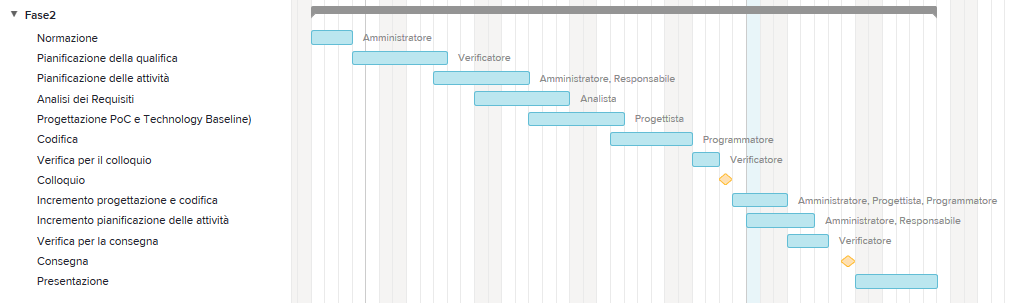
\includegraphics[scale=0.67]{images/fase2.png}
	\caption{Diagramma di Gantt riguardante la fase 2}
\end{figure}